%!TEX root = ../thesis.tex
%*******************************************************************************
%****************************** Third Chapter **********************************
%*******************************************************************************
\chapter{Phase Transition}

% **************************** Define Graphics Path **************************
\ifpdf
    \graphicspath{{Chapter3/Figs/thermodynamics/}{Chapter3/Figs/}}
\else
    \graphicspath{{Chapter3/Figs/thermodynamics/}{Chapter3/Figs/}}
\fi

\textbf{What is this}
Phase transition is one of the most studied problem in physics. Phase transition is a process where below a critical point the system behaves in one way whereas above that point the system behaves in a completely different way. There is a control parameter in phase transition. It can be temperature $T$ or magnetic field $H$. For example in ferromagnet to paramagnet transition temperature is the control parameter and for normal to superconductor transition both temperature and magnetic field are the control parameter.\\
The first explicit statement of the first law of thermodynamics, by \textit{Rudolf Clausius} in 1850, referred to cyclic thermodynamic processes. \\
\textit{In all cases in which work is produced by the agency of heat, a quantity of heat is consumed which is proportional to the work done; and conversely, by the expenditure of an equal quantity of work an equal quantity of heat is produced.}\\
\begin{align}
	\Delta E = Q + W
\end{align}
where, $Q$ is the net quantity of heat supplied to the system by its surroundings and $W$ is the net work done by the system.
The IUPAC convention for the sign is as follows: All net energy transferred to the system is positive and net energy transferred from the system is negative.
Clausius also stated the law in another form, referring to the existence of a function of state of the system, the internal energy, and expressed it in terms of a differential equation for the increments of a thermodynamic process.\\
\textit{In a thermodynamic process involving a closed system, the increment in the internal energy is equal to the difference between the heat accumulated by the system and the work done by it.}\\
For quasi-static process
\begin{align}
	dE = dQ - P dV
\end{align}
$E$ is the internal energy.
here $W = -P dV$
since work done by the system on the environment if the product $P dV$ whereas the work done on the system is $-P dV$ for pressure $P$ and volume change $dV$.\\
The term heat for $Q$ means "that  amount of energy added or removed by conduction of heat or by thermal radiation", rather than referring to a form of energy within the system. 
The internal energy is a mathematical abstraction that keeps account of the exchanges of energy that befall the system.

For quasi-static state we can write
\begin{equation}
dQ = T dS
\ref{eqn:def_enthalpy}
\end{equation}
where $S$ is the entropy of the system and $T$ is the temperature.
Thus we can write for canonical ensemble
\begin{equation}
dE = TdS - pdV
\end{equation}
such that $E=E(S,V)$  and 
for grand canonical ensemble 
\begin{equation}
dE = TdS - pdV + \mu dN
\end{equation}
where $E=E(S,V,N)$.
But a problem arises, since there is no device we currently posses that can measure entropy. So we use Legendre transformation to change variable dependency
\begin{align}
	dE  	&= TdS - pdV  \nonumber \\ 
	&= TdS + SdT - SdT - PdV  \nonumber \\ 
	d(E-TS) &= -SdT - PdV  \nonumber \\
	dA 		&= -SdT - PdV \label{eqn:helmholtz_def}
\end{align}
where $A=A(T,V)$  is the Helmholtz free energy. We can perform another Legendre transformation in \ref{eqn:helmholtz_def} as follows
\begin{align}
	dA 		&= -SdT - PdV -VdP + VdP \nonumber \\
	d(A+PV) &= -SdT + VdP \nonumber \\
	dG      &= -SdT + VdP \label{eqn:gibbs_def}
\end{align}
where $G=G(T,P)$ is the Gibbs free energy.\\
Let's take a break to talk about free energy. What is free energy?
\section{Classification}
	\subsection{First Order}
		\begin{enumerate}
			\item Latent heat of nucleation in growth
			\item Symmetry may or may not be broken
			\item Discontinuous change in entropy
		\end{enumerate}
	\subsection{Second Order}
		\begin{enumerate}
			\item Sysmmetry is always broken
			\item No Latent heat or meta-stable state
			\item Continuous change in entropy
		\end{enumerate}
	
\section{Thermodynamic Quantities}
	\subsection{Entropy}
	\label{subsect:entropy-thermodynamics}
	One of the most important concept in Statistical Mechanics is entropy. The notion of entropy was first introduced in physics by a German scientist Rudolf Clausius who laid the foundation for the second law of thermodynamics in 1850 by examining the relation between heat transfer and work.
	The second law of thermodynamics states that the total entropy of an isolated system can never decrease over time. Therefore the direction toward which entropy increases monotonically is the direction of time. Monotonically means that it can increase or keep constant but never decrease. 
	The term entropy	is used in many other branches of science, sometimes distant from physics or mathematics (such	as sociology), where it no longer maintains its rigorous quantitative character. Usually, it roughly	means disorder, chaos, decay of diversity or tendency toward uniform distribution of kinds \cite{Downarowicz2009}.
	
	Entropy is considered as a quantity about the disorderness of a system. This kind of disorder is the number of states a system can take on. So what are the states of a system? Imagine a cube of volume $1cm^3$, filled with one particular gas. At a particular time if we can label all the molecules of the gas uniquely then at next moment most of the molecule will change their positions due to their random motion. Then we will not be able to identify each molecule with their previous label. This process of identifying the labels of the molecules are easier if it's a liquid and even more easier in it's solid form. Since temperature increases the random motion of the molecules, as the temprature rises it is more difficult to identify those molecules. Thus at high temperature a system has higher entropy. Another thing to mention about it's volume. If a larger volume is selected then obviously the number of possible states will increase therefore entropy will increase.\\
	Example:\\
	If we were ot compare the entropy of the moon and the sun, the above discussion tells us that the sun has higher entropy than the moon. The reason is that the sun is much much larger than the moon and has much higher temperature than the moon. Therefor the number of possible states will be larger for the sun than the moon.\\
	
	In Classical Physics, entropy is seen as a magnitude which in every time is proportional to	the quantity of energy that at that time cannot be transformed into mechanical work. Using the	above interpretation, entropy plays a central role in the formulation of the second law of thermodynamics which states that in an isolated physical system, any transformation leads to an increase	of its entropy. 
	
	In Probability Theory, the entropy of a random variable measures the uncertainty over the	values which can be reached by the variable.
	
	In Information Theory, the entropy of the compression of a message (for example, of a file	from a computer), quantifies the content of the information of the message to have the minimum	lost of information in the compression process previous to its transmission.
	
	In Abstract Theory of Dynamical Systems, the entropy measures the exponential complexity	of the system or the average flow of information per unit of time \cite{Balibrea2016}.
	
	So it is already explicit that the concept of entropy is not easy to grasp and frequently entropy is seen as very mysterious quantity and that’s why it received a very large number of interpretations,
	explications, applications. In order to understand how the complex concept of entropy emerged,
	in this chapter we will give a brief history and will review the works of Clausius, Boltzmann,
	Shannon and Rényi.

	\subsubsection{Clausius Entropy}	
	As mentioned Earlier in this section The concept and name of entropy originated in the early
	1850s in the work of Rudolf Julius Emmanuel Clausius $(1822-1888)$ and that work was at first	primarily concerned with the question of which cycle is best suited for the conversion of heat into	work and which substance is best used for the conversion \cite{Clausius1867}.
	
	Clausius based his argument on the plausible axiom that heat cannot pass by itself from a cold to a hot body. In order to exploit that axiom Clausius considered two competing Carnot cycles (see figure	\ref{fig:carnot-engines}) working in the same temperature range, one as a heat engine and one as a refrigerator;	the refrigerator consumes the work the engine provides. By comparing the amounts of heat $Q$	passed from top to bottom and vice versa, he came to the conclusion that among all efficiencies	the efficiency of a Carnot cycle is maximum and universal.	'Maximum' means that no cycle in the same range of temperature has a bigger efficiency than a	Carnot cycle, and 'universal' means that all working substances provide the same efficiency in a	Carnot cycle \cite{Carnot1890}.	It is easy to calculate the efficiency of the Carnot engine of an ideal gas:
	\begin{figure}
		\centering
		\includegraphics[width=10cm]{{{carnot-cycle-heat-engine-refrigerator}}}
		\caption{Two competing Carnot engines, pressure (P) versus volume (V) - diagrams \cite{Greven2003}}
		\label{fig:carnot-engines}
	\end{figure}
	\begin{align}
		\eta &= \frac{W}{Q_{boiler}} \nonumber\\
		     &= \frac{Q_{boiler} - Q_{cooler}}{Q_{boiler}} \nonumber\\
		     &= 1 - \frac{Q_{cooler}}{Q_{boiler}} \\
		     &= 1 - \frac{T_{cooler}}{T_{boiler}}
		     \label{eqn:efficiency-carnot}
	\end{align}
	where $T$ is the Kelvin temperature. And, since by Clausius’ result this efficiency is universal, it	holds not only for ideal gases but for all substances, be they water, mercury, sulphur, or steel.
	Nicolas L\'{e}onard Sadi Carnot anticipated Clausius by 30 years, but no one could understand	Carnot's reasoning. Carnot believed in the caloric theory of heat, by which the heat passing through	the cycle from boiler to cooler is unchanged in amount. This is quite wrong and it is a kind of miracle that Carnot, despite his erroneous concepts, obtained a correct result. Carnot's trouble was	that he did not know the balance of energy, or the first law of thermodynamics, which states that
	\begin{align}
		dU &= dQ - dW \\
		   &= dQ - P dV
	\end{align}
	since
	\begin{equation}
		dW = P dV
	\end{equation}
	This equation holds, if the work is expended reversibly for the volume change. With that superior	knowledge Clausius showed that it is not the heat that passes through the cycle from boiler to	cooler unchanged in amount. He proved that from equation \ref{eqn:efficiency-carnot}
	\begin{equation}
		\frac{Q}{T}\at[\Big]{\text{boiler}} =
		\frac{Q}{T}\at[\Big]{\text{heater}}
	\end{equation}
	nd decided to define the entropy change to be the ratio of heat flow to temperature: \cite{Sethna2006}
	\begin{equation}
		\Delta S_{\text{thermo}} = \frac{Q}{T}
	\end{equation}
	He also showed that in an arbitrary process, the change of entropy, satisfies the inequality
	\begin{equation}
		dS \geq \frac{dQ}{T}
		\label{eqn:2nd-law-of-themodynamics}
	\end{equation}
	This important relation is known as the second law of thermodynamics. We will now discuss the significance of this law.
	First, we stick to reversible process, where the equality holds in equation \ref{eqn:2nd-law-of-themodynamics}. We may then eliminate $dQ$ between the first and second laws, we obtain the Gibbs equation
	\begin{equation}
		dS = \frac{1}{T} \left(dU + P dV\right)
	\end{equation}
	In an adiabatic irreversible process, $dQ = 0$ and equation \ref{eqn:2nd-law-of-themodynamics} one has the fundamental relation between entropy and irresponsibility. In words\\
	\textbf{In a closed system (adiabatic), the entropy cannot decrease, it remains constant or increase \cite{Benguigui2013}}
	But the irreversible increase of entropy is not a property of the microscopic laws of nature. Because the microscopic laws of nature are time-reversal invariant. For example the Maxwell's equations are time reversible or the laws governing the motion of electrons of atoms are also time reversible. Thus the direction of time cannot be determined from microscopic laws of nature. But since entropy always increase monotonically, the direction in which entropy increases (or remains constant) is the direction of time \cite{Sethna2006}.
	%----------------------------------------------
	\subsubsection{Boltzmann Entropy}
	Another intuitive interpretation of entropy is as a measure of the disorder in a system.  Liquids have higher entropy	than crystals intuitively because their atomic positions are less orderly \cite{Sethna2006}. Ludwig Boltzmann	interpreted the entropy function as statistical entropy using probability theory.	Around 1900 there was a fierce debate going on between scientists whether atoms really existed	or not. Boltzmann was convinced that they existed and realized that models that relied on atoms	and molecules and their energy distribution and their speed and momentum, could be of great	help to understand physical phenomena. Because atoms where supposed to be very small, even	in relatively small systems, one faces already a tremendous number of atoms. For example: one
	mole of water contains about $6.023 \times 10^{23}$ molecules! Clearly it is impossible to track the energy	and velocity of each individual atom. Therefore, Boltzmann introduced a mathematical treatment	using statistical mechanical methods to describe the properties of a given physical system (for example the relationship between temperature, pressure and volume of one liter of air). 
	
	Boltzmann's	idea behind statistical mechanics was to describe the properties of matter from the mechanical	properties of atoms or molecules. In doing so, he was finally able to derive the Second Law of	Thermodynamics around 1890 and showed the relationship between the atomic properties and the	value of the entropy for a given system. It was Max Planck who formulated the expression of entropy of the ideal gas system based on Boltzmann’s results \cite{Schmitz2007}. The Boltzmann entropy formula	or Boltzmann-Planck entropy formula is
	\begin{equation}
		S = k_B \log\Omega
		\label{eqn:boltzmann-entropy}
	\end{equation}

	$S$ is called the Planck entropy or Boltzmann entropy. Here $k_B$ is the Boltzmann constant
	(ideal gas constant $R$ divided by Avogadro's number $N$) which equals to $1.4 \times 10^{-23}$ $J/K$), and $\Omega$, comes from the German \textit{Wahrscheinlichkeit}, meaning probability, which is often referred to as	disorder. In another way we can define it as the number of microstates (often modeled as quantum	states) with the given macrostate. Macrostate is any particular arrangement of atoms where we	look only on average quantities. Any individual arrangement defining the properties (e.g. positions	and velocities) of all the atoms for a given macrostate is a microstate. For a microstate it matters	what individual particles do, for the macrostate it does not.
	
	
	The logarithm is used because it simplifies the computations and reproduced the property of additivity of entropy, in the sense that the entropy of two systems sums instead of multiplies. In	equation \ref{eqn:boltzmann-entropy}, the entropy $S$ increases when $\Omega$ does. The more microstates are, the more disorder	and more entropy are. Besides for only one possible microstate, entropy is zero. The notion of	disorder is an intuitive notion depending of the system to be considered. In the case of a gas, it	is considered it in a ordered state if its molecules have a distribution of energies or positions very	different of those random which means the Boltzmann distribution. The most disordered states are	the most probable and as consequence have the most entropy. Another consequence is that in the	universe the disorder tends to increase \cite{Balibrea2016}.
	
	
	From there, it is a short conceptual jump to the second Law (total entropy tends to increase, and	all spontaneous processes increase entropy). In summary, the thermodynamic definition of entropy provides the experimental definition of entropy, while the probabilistic definition of entropy	extends the concept, providing an explanation and a deeper understanding of its nature \cite{Alam2016}.
	
	These definitions of entropy is of no use in our model. However we can use the Boltzmann entropy with a few modification to get Shannon entropy \cite{shanon_entropy}. This process of getting Shannon entropy from Boltzmann entropy and how does it help us is described in section \ref{subsect:percolation-entropy}.
	
	\subsection{latent heat}
	The latent heat associated with the phase transition is , where and are the entropies just above and below the phase transition. Since the entropy is continuous at the phase transition, the latent heat is zero. The latent heat is always zero for a second order phase transition.
	\subsection{Specific Heat}
	The specific heat is the amount of heat per unit mass required to raise the temperature by one degree Celsius. The relationship between heat and temperature change is usually expressed in the form shown below where $C$ is the specific heat.
	\begin{equation}
		C = \frac{Q}{dT}
	\end{equation}
	and we know
	\begin{equation}
		Q = T dS
	\end{equation}
	where $S$ is the entropy. we immediately get
	\begin{equation}
		C = T \frac{dS}{dT}
		\label{def:specific-heat-thermodynamics}
	\end{equation}
	
	\subsection{Order Parameter}
	\subsection{Susceptibility}
	The first law of thermodynamics for a non magnetic system is \ref{label}
	\begin{equation}
		dE = TdS - PdV
	\end{equation}
	for a magnetic system $P \rightarrow h$ and $V \rightarrow -m$, where $h$ is the magnetic field and $m$ is the magnetization. The negative sign for the magnetization is because of the fact that the magnetization increases with the increase of the magnetic field whereas the volume decreases as the pressure increases. Since we relate pressure to the magnetic field, to relate volume to magnetization we need to put a minus sign with it. Thus we get
	\begin{align}
		dE &= TdS + hdm \\
		   &= TdS + SdT - SdT + h dm \\
		d(E - TS)  &= -SdT + h dm \\
		dA &= -SdT + h dm \label{eqn:helmholtz_mag_system} \\
		dA &= -SdT + h dm + m dh -m dh \\
		d(A - mh) &= -SdT - m dh\\
		dG &= -SdT -m dh \label{eqn:gibbs_mag_system}
	\end{align} 
	where $A=A(T,m)$ is the  Helmholtz free energy and $G=G(T,h)$ is the Gibbs free energy for the magnetic system. From the definition of free energy for a magnetic system \ref{eqn:gibbs_mag_system} \ref{eqn:helmholtz_mag_system} we can find the expression for entropy and magnetization in terms of free energy.
	\begin{equation}
		S = -\left(\frac{\partial G}{\partial T}\right)_h = -\left(\frac{\partial A}{\partial T}\right)_m
	\end{equation}
	\begin{equation}
		m = -\left(\frac{\partial G}{\partial h}\right)_T
		\label{eqn:magnetization_def}
	\end{equation}
	\begin{equation}
		h = \left(\frac{\partial A}{\partial m}\right)_T
		\label{eqn:mag_field_def}
	\end{equation}	
	And since the susceptibility is defined as the derivative of the magnetization with respect to the magnetic field, we get
	\begin{equation}
		\chi = \left(\frac{\partial m}{\partial h}\right)_h = - \left(\frac{\partial^2G}{\partial h ^2}\right)_T
		\label{eqn:susceptibility_def}
	\end{equation}
	again we can write $\chi$ as
	\begin{align}
		\chi &= \frac{1}{\frac{\partial h}{\partial m}} \nonumber \\
			 &= \frac{1}{\frac{\partial^2 A}{\partial m ^2}} \label{eqn:susceptibility_def2}
	\end{align}
	
	
	%-------------------------------------------------------------------------------------------
\section{Shapes of the Thermodynamic Quantities}
	\subsection{Calculus to determine the shapes}
	\label{sec:determine_shape_using_calculus}
	From the law of Calculus we can estimate the approximate shape of a function by it's first and second derivative.
	Say we have a function $f(x)$ and we want to estimate it's shape.
	If the first derivative of this function is negative (positive) the function is said to have decreasing (increasing) slope \ref{fig:diff1_of_f}.
	\begin{figure}
		\centering
		\begin{subfigure}{0.329\textwidth}
			\centering
			\includegraphics[width=\linewidth]{{{thermodynamics/decreasing}}}
			\caption{negative slope}
		\end{subfigure}
		\begin{subfigure}{0.329\textwidth}
			\centering
			\includegraphics[width=\linewidth]{{{thermodynamics/increasing}}}
			\caption{positive slope}
		\end{subfigure}
		\caption{shape of $f(x)$ from $f^{\prime}(x)$}
		\label{fig:diff1_of_f}
	\end{figure}
	
	If the second derivative of this function is negative (positive) the function is said to have concave (convex) shape \ref{fig:diff2_of_f}.
	\begin{figure}
		\centering
		\begin{subfigure}{0.329\textwidth}
			\centering
			\includegraphics[width=\linewidth]{{{thermodynamics/concave}}}
			\caption{concave}
		\end{subfigure}
		\begin{subfigure}{0.329\textwidth}
			\centering
			\includegraphics[width=\linewidth]{{{thermodynamics/convex}}}
			\caption{convex}
		\end{subfigure}
		\caption{shape of $f(x)$ from $f^{\prime\prime}(x)$}
		\label{fig:diff2_of_f}
	\end{figure}
	Thus if we know the sign of the first and second derivative we can approximate a shape of the function.
	\subsection{Free Energy}
	Now since we obtain from \ref{eqn:gibbs_def} that the entropy is the first derivative of the free energy \ref{eqn:entropy_by_gibbs} and from \ref{eqn:def2_specific_heat} specific heat is the second derivative of the free energy \ref{eqn:specific_heat_by_gibbs}. Now since the entropy is a positive quantity and specific heat is also a positive quantity we get that the first and second derivative of the free energy is negative which implies from the laws of calculus that the shape of the free energy should be a decreasing concave curve \ref{fig:free_energy} in other words concave shaped with negative slope.
	\begin{equation}
	S = - \frac{\partial G}{\partial T}
	\label{eqn:entropy_by_gibbs}
	\end{equation}
	\begin{equation}
	C = - \frac{\partial^2 G}{\partial T ^2}
	\label{eqn:specific_heat_by_gibbs}
	\end{equation}
	\begin{figure}
		\centering
		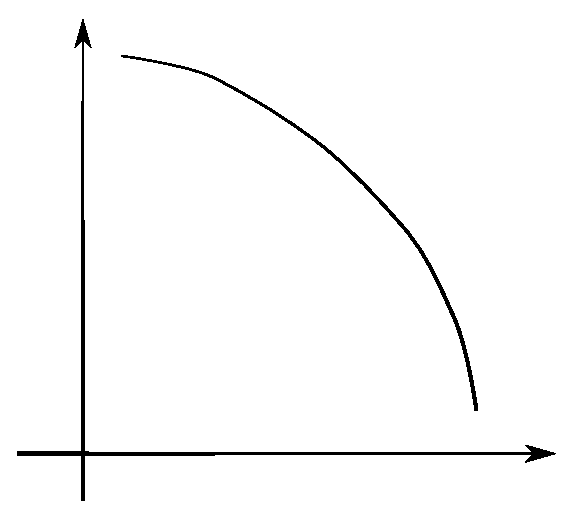
\includegraphics[width=0.3\columnwidth]{{{thermodynamics/free_energy}}}
		\caption{Shape of the free energy}
		\label{fig:free_energy}
	\end{figure}

	\subsection{Entropy and Specific Heat}	
	Now that we know the shapes of the free energy, the very next thing to do is to find the shape of the entropy. Since we can get entropy from differentiating the free energy with respect to temperature $T$ we get the following shape \ref{fig:entropy_1_2}. From the definition of the transition order we know that the first order transition is discontinuous and the second order transition continuous. Since the first order transition requires latent heat at the critical point the discontinuity is inevitable. Note that, since entropy measures disorderedness of a system it should increase with increasing temperature. Because the temperature is nothing but the average kinetic energy of the particles in the system. As the kinetic energy of the system increases with temperature, the particles tend to vibrate more and get higher average velocity. Thus making the system disordered. Therefore in a physical system entropy always increases with the increasing of temperature. If we find something different, as if, the entropy is decreasing with the increasing of temperature, there must be a problem somewhere.
	\begin{figure}
		\centering
		\begin{subfigure}{0.329\textwidth}
			\centering
			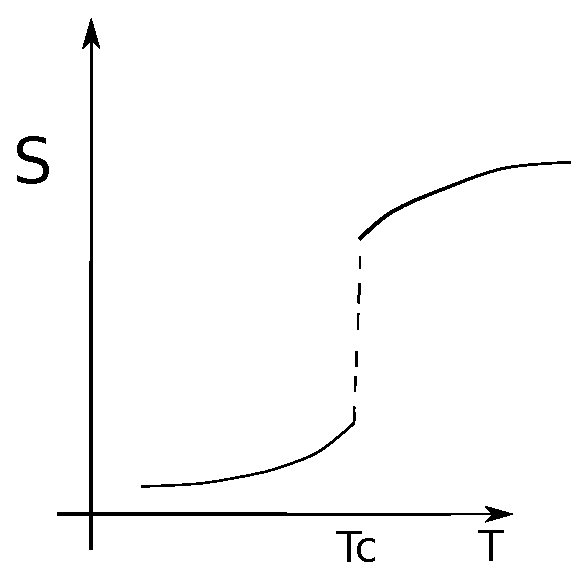
\includegraphics[width=\linewidth]{{{thermodynamics/entropy_1st}}}
			\caption{Entropy in first order transition}
		\end{subfigure}
		\begin{subfigure}{0.329\textwidth}
			\centering
			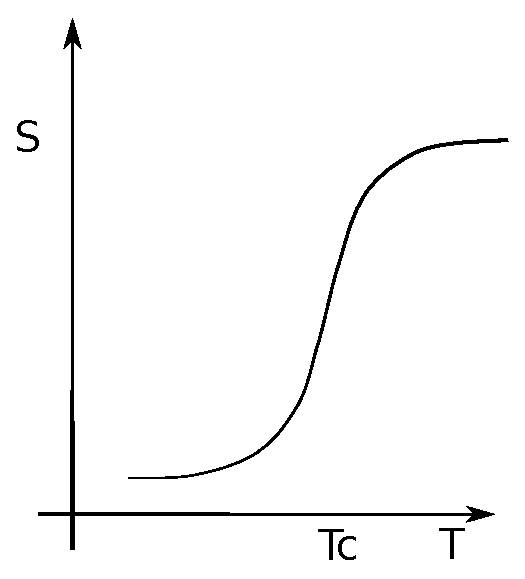
\includegraphics[width=\linewidth]{{{thermodynamics/entropy_2nd}}}
			\caption{Entropy in 2nd order transition}
		\end{subfigure}
		\caption{Shape of entropy}
		\label{fig:entropy_1_2}
	\end{figure}
	Just after knowing the shape of entropy one can anticipate the shape of specific heat, which is the derivative of the entropy with respect to temperature and is defined in \ref{eqn:def2_specific_heat_by_entropy}. Using this and the shape of entropy we can get the shape of the specific heat immediately as follows
	\begin{figure}
		\centering
		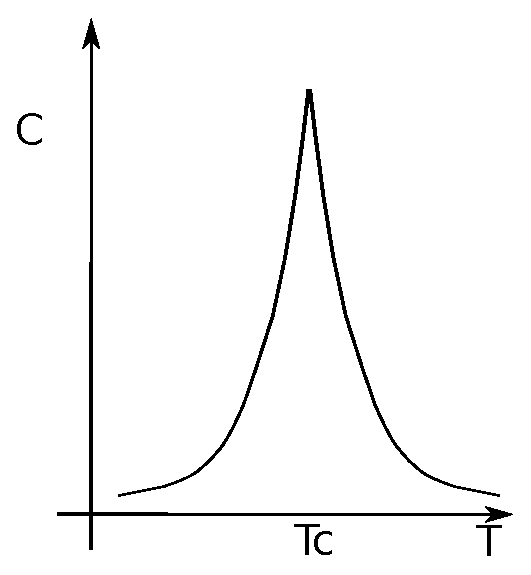
\includegraphics[width=\linewidth]{{{thermodynamics/specific_heat}}}
		\caption{Shape of Specific Heat}
		\label{fig:specific_heat}
	\end{figure}
	\subsection{Order Parameter and Susceptibility}
	Since diamagnetic substances have negative susceptibilities $(\chi < 0)$; paramagnetic, and ferromagnetic substances have positive susceptibilities $(\chi > 0)$, and we are working for a phase transition model similar to paramagnet and ferromagnet transition, taking susceptibility to be positive is appropriate for our model. Now if susceptibility is positive then from \ref{eqn:susceptibility_def} we get $\left(\frac{\partial^2G}{\partial h ^2}\right) < 0$ which means that the shape of the free energy for this case is concave from the knowledge of \ref{sec:determine_shape_using_calculus}. And from \ref{eqn:magnetization_def} and the fact that the magnetic field $h$ can be positive or negative, as it can change direction, the Gibbs free energy is negative, since it is the lowest binding energy. \\
	Also from \ref{eqn:susceptibility_def2} we can say $\frac{\partial^2 A}{\partial m ^2}$ is positive giving convex shape of the Helmholtz free energy. And \ref{eqn:mag_field_def} tells us that since $h$ can ve positive or negative, the Helmholtz free energy can have increasing or decreasing slope respectively.
	\begin{figure}
		\centering
		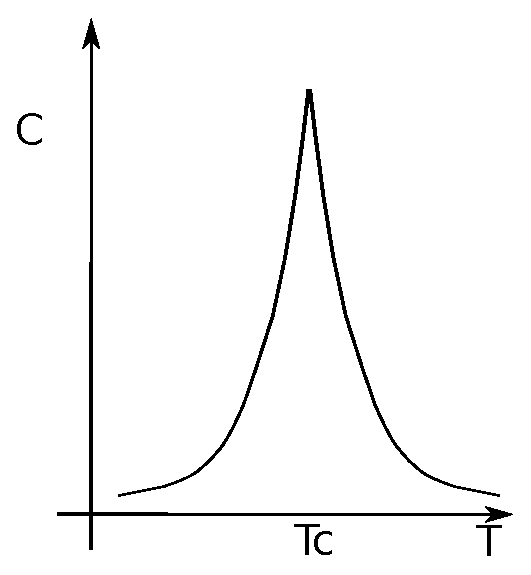
\includegraphics[width=\linewidth]{{{thermodynamics/specific_heat}}}
		\caption{figure required}
	\end{figure}
	


%-----------------------------------------------------------------------------------
\section{Response Functions}
The Specific heat and Susceptibility are called the response function in thermodynamics and the definitions are as follows. The specific heat $C_p$ or $C_v$ is the derivative of the enthalpy with respect to the temperature at constant pressure or volume respectively.
\begin{equation}
C_x = \left(\frac{dQ}{dT}\right)_x
\label{eqn:def_specific_heat}
\end{equation}
here $x$ can be $P$ for pressure or $V$ for volume. And from \ref{eqn:def_enthalpy} we can write
\begin{equation}
C_x = T \left(\frac{dS}{dT}\right)
\label{eqn:def2_specific_heat_by_entropy} 
\end{equation}
To give the following
\begin{align}
C_v = -T\left(\frac{\partial^2 A}{\partial T^2}\right)_v \\
C_p = -T\left(\frac{\partial^2 G}{\partial T^2}\right)_p
\label{eqn:def2_specific_heat} 
\end{align}

Nearest neighbor interation and 2nd nearest neighbor interaction.
Old models of phase transition : Ising model 1D and 2D. Bragg Willium model. 

%------------------------------------------------------------------------------------
\section{Critical Exponents}
	Near the critical point there is, in general, a function that describes the behavior of the system that is mostly interesting. For thermodynamical system the temperature is the control parameter \ref{??}, thus that function depends on the temperature. But since we want the information at the critical point, $(T-T_c)/T_c$, instead of $T$ is a better parameter to address. In equation
	\begin{equation}
		\epsilon = \frac{T-T_c}{T_c} = \frac{T}{T_c} - 1
	\end{equation}
	$\epsilon$ is considered a better parameter. Thus a function $f(\epsilon)$ is used instead of $f(T)$. Using the fact that near $T_c$ the function $f(\epsilon)$ exhibits power law \ref{??}
	\begin{equation}
		f(\epsilon) \sim \epsilon^\lambda
	\end{equation}
	The following figures shows some function that exhibit power law
	\begin{figure}
		\centering
		\begin{subfigure}{0.4\textwidth}
			\centering
			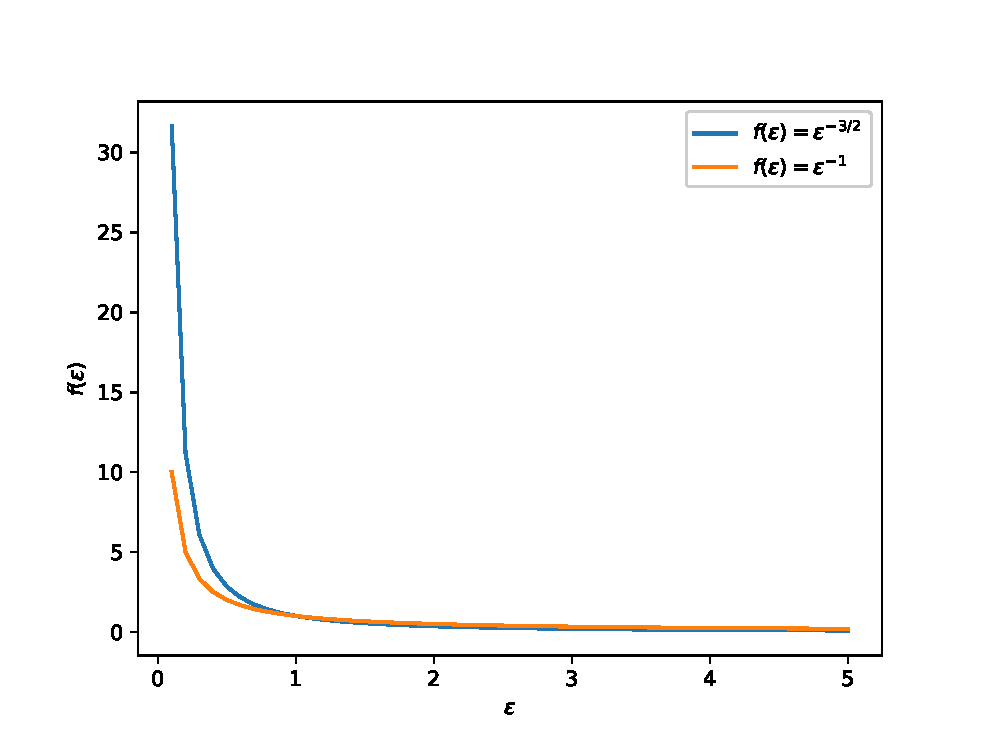
\includegraphics[width=\linewidth]{{{power_law_functions/fig1}}}
			\caption{$f(\epsilon) \sim \epsilon^\lambda$ where $\lambda=-1,-3/2$}
		\end{subfigure}
		\begin{subfigure}{0.4\textwidth}
			\centering
			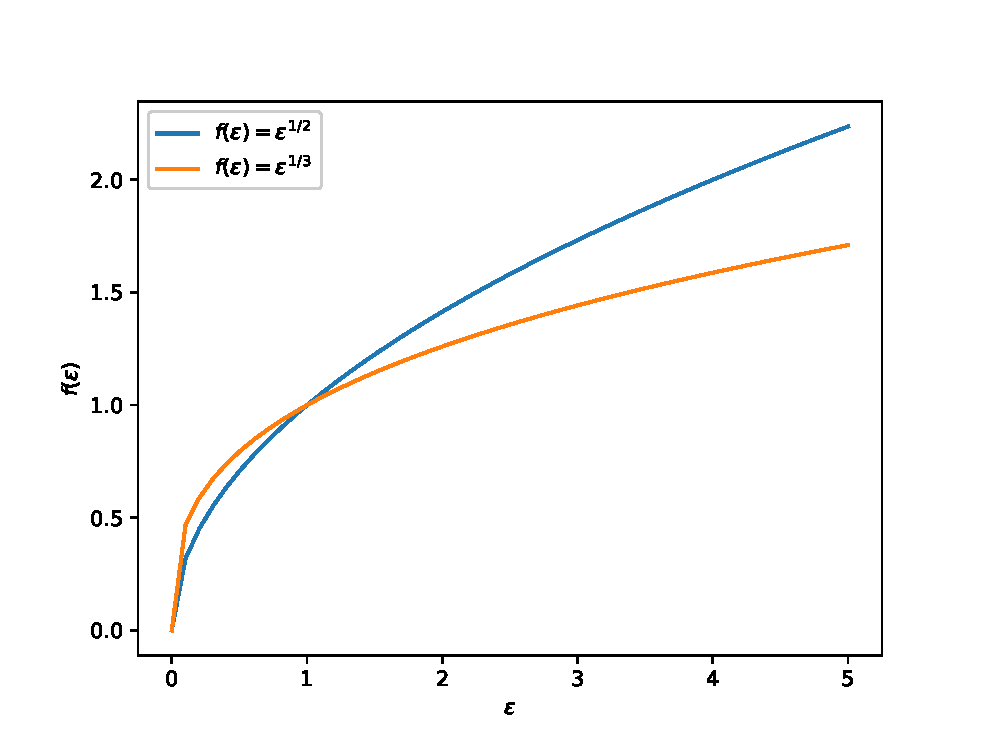
\includegraphics[width=\linewidth]{{{power_law_functions/fig2}}}
			\caption{$f(\epsilon) \sim \epsilon^\lambda$ where $\lambda=1/2,1/3$}
		\end{subfigure}
		\caption{Function showing power law}
	\end{figure}
	To see this more closely, we can expand any function $f(\epsilon)$ as a power series of $\epsilon$
	\begin{equation}
		f(\epsilon) = A \epsilon^\lambda ( 1 + B \epsilon^a + C \epsilon^b + ...)
	\end{equation}
	Near $T_c$ only the first term is dominating \ref{??}.\\
	We had the Gibbs free energy (for a magnetic system)
	\begin{equation}
		G = G(T,h) \equiv G(\epsilon, h)
	\end{equation}
	since $\epsilon$ is a better parameter. Assume that $G$ is a generalized Homogeneous function. Therefore from \ref{??} we can write
	\begin{equation}
		G(\lambda^{a_\epsilon} \epsilon, \lambda^{a_h} h) = \lambda G(\epsilon, h)
		\label{eqn:gibbs_homogenious}
	\end{equation}
	differentiating equation \ref{eqn:gibbs_homogenious} with respect to $h$
	\begin{align}
		\frac{\partial G(\lambda^{a_\epsilon} \epsilon, \lambda^{a_h} h)}{\partial h} &= \lambda \frac{\partial G(\epsilon, h)}{\partial h} \nonumber \\
		\frac{\partial G(\lambda^{a_\epsilon} \epsilon, \lambda^{a_h} h)}{\partial \lambda^{a_h} h} \lambda^{a_h} &= \lambda \frac{\partial G(\epsilon, h)}{\partial h} \nonumber \\
		\lambda^{a_h} G^\prime(\lambda^{a_\epsilon} \epsilon, \lambda^{a_h} h) &= \lambda G^\prime (\epsilon, h) \nonumber \\
		-\lambda^{a_h} m(\lambda^{a_\epsilon} \epsilon, \lambda^{a_h} h) &= -\lambda m(\epsilon, h) \nonumber \\
		m(\lambda^{a_\epsilon} \epsilon, \lambda^{a_h} h) &= \lambda^{1-a_h} m(\epsilon, h) \\
		\label{eqn:order_parameter_homogeneous}
	\end{align}
	Here $m$ is the magnetization or order parameter.\\
	\textbf{Figure of order general parameter}\\
	Setting $h=0$ in equation \ref{eqn:order_parameter_homogeneous}
	\begin{align}
		m(\lambda^{a_\epsilon} \epsilon)	 &= \lambda^{1-a_h} m(\epsilon) \nonumber \\
		m(1)	 &= \lambda^{1-a_h} m(\epsilon) \nonumber \\
		m(1)	 &= \epsilon^{-\frac{1-a_h}{a_\epsilon}} m(\epsilon) \nonumber \\
		m(\epsilon) &= \epsilon^\beta m(1) \label{eqn:order_parameter_and_beta}
	\end{align}
	where
	\begin{equation}
		\beta = \frac{1-a_h}{a_\epsilon}
		\label{eqn:beta}
	\end{equation}
	Note that, setting $\lambda^{a_\epsilon} \epsilon = 1$ gives $\lambda = \epsilon^{-1/a_\epsilon}$.\\
	Setting $\epsilon=0$ in equation \ref{eqn:order_parameter_homogeneous}
	\begin{align}
		m(\lambda^{a_h} h) &= \lambda^{1-a_h} m(h) \nonumber \\
		m(1) &= h^{-\frac{1-a_h}{a_h}} m(h) \nonumber \\
		m(h) &= m(1) h^\delta \label{eqn:order_parameter_and_delta}
	\end{align}
	where
	\begin{equation}
		\delta = \frac{a_h}{1-a_h}
		\label{eqn:delta}
	\end{equation}
	Again, note that, setting $\lambda^{a_h} h = 1$ gives $\lambda = h^{-1/a_h}$\\
	Now, Since the response functions are the second derivative of the free energy \ref{??}, by differentiating \ref{eqn:gibbs_homogenious} twice with respect to $\epsilon$ we get the Specific Heat
	\begin{align}
		\lambda^{2 a_\epsilon} G^{\prime\prime}(\lambda^{a_\epsilon} \epsilon, \lambda^{a_h} h) &= \lambda G^{\prime \prime}(\epsilon, h) \nonumber \\
		\lambda^{2 a_\epsilon} \frac{\partial G(\lambda^{a_\epsilon} \epsilon, \lambda^{a_h} h)}{\left(\frac{1}{T_c}\right)^2 \partial T^2} &= \lambda G^{\prime \prime}(\epsilon, h) \nonumber \\
		\lambda^{2 a_\epsilon} C(\lambda^{a_\epsilon} \epsilon, \lambda^{a_h} h) &= \lambda C(\epsilon, h)
		\label{eqn:specific_heat_homogeneous}
	\end{align}
	We have used $\epsilon = \frac{T}{T_c} -1$ and $d\epsilon = \frac{1}{T_c} dT$. Now setting $h=0$ we get from \ref{eqn:specific_heat_homogeneous}
	\begin{align}
		\lambda^{2 a_\epsilon} C(\lambda^{a_\epsilon} \epsilon) &= \lambda C(\epsilon) \nonumber \\
		C(1) &= \lambda^{1- 2 a_\epsilon} C(\epsilon) \nonumber \\
			 &= \epsilon^{-\frac{1-2 a_\epsilon}{a_\epsilon}} C(\epsilon) \nonumber \\
		C(\epsilon) &= \epsilon^{-\alpha} C(1) \label{eqn:specific_heat_and_alpha}
	\end{align}
	We have used the value of $\lambda$ when we set $\epsilon \lambda^{a_\epsilon}=1$ and the exponent
	\begin{equation}
		\alpha = \frac{2 a_\epsilon - 1}{a_\epsilon}
		\label{eqn:alpha}
	\end{equation}
	
	Again by differentiating \ref{eqn:gibbs_homogenious} twice with respect to $h$ we get the susceptibility. Then we set $h=0$ to get only $\epsilon$ dependency.
	\begin{align}
		\lambda \frac{\partial^2 G(\epsilon,h)}{\partial h^2} &= \lambda^{2 a_h} \frac{\partial^2 G(\lambda^{a_\epsilon} \epsilon, \lambda^{a_h} h)}{\partial h^2} \nonumber \\
		\lambda \chi(\epsilon, h) &= \lambda^{2 a_h} \chi(\lambda^{a_\epsilon}\epsilon, \lambda^{a_h} h) \nonumber \\
		\chi(\epsilon) &= \lambda^{2 a_h - 1} \chi(\lambda ^{a_\epsilon} \epsilon) \nonumber \\
		\chi(\epsilon) &= \epsilon^{-\gamma} \chi(1) 
		\label{eqn:susceptibility_homogeneous}
	\end{align}
	Similar to previous case, We have used the value of $\lambda$ when we set $\epsilon \lambda^{a_\epsilon}=1$ and the exponent is
	\begin{equation}
		\gamma = \frac{2 a_h -1}{a_\epsilon}
		\label{eqn:gamma}
	\end{equation}
	\subsection{List of Thermodynamic Quantities that Follows Power Law}
	\textbf{Critical Exponents at a glance} is it better title.\\
		The exponent that scales Specific heat is called $\alpha$ 
		\begin{equation}
			C \sim \epsilon^{-\alpha}
		\end{equation}
		The exponent that scales order-parameter is called $\beta$ 
		\begin{equation}
			m \sim \epsilon^{\beta}
		\end{equation}
		Another exponent that scales order-parameter is called $\delta$, but it relates the order parameter with the magnetic field, $h$
		\begin{equation}
			m \sim h^{\delta}
		\end{equation}
		The exponent that scales susceptibility is called $\gamma$ 
		\begin{equation}
			\chi \sim \epsilon^{-\gamma}
		\end{equation}
		Note that these quantities only follows power law near $T_c$.
	\subsection{Rushbrooke Inequality}
		\begin{equation}
			\alpha + 2 \beta + \gamma \ge 2
		\end{equation}
		but the equality is often obtain theoretically which is shown below in the present case 
		\begin{align}
			\alpha + 2\beta + \gamma &= \frac{2 a_\epsilon -1}{a_\epsilon} 
					+ \frac{2 (1 - a_h)}{a_\epsilon}
					+ \frac{2 a_h - 1}{a_\epsilon} \nonumber \\
					&= \frac{2 a\epsilon}{a\epsilon} \nonumber \\
					&= 2 \nonumber
		\end{align}
	Thus the Rushbrooke inequality is satisfied.
	\subsection{Griffiths Inequality}
	\begin{equation}
		\alpha + \beta (1+\delta)  = 2
	\end{equation}
	Let's do a quick check to see if this is also satisfied.
	\begin{align}
		\alpha + \beta (1+\delta) &= \frac{2 a_\epsilon - 1}{a_\epsilon} 
									+ \frac{1 - a_h}{a_\epsilon} \left(1 + \frac{a_h}{1 - a_h}\right) \nonumber \\
								  &= \frac{2 a_\epsilon - 1}{a_\epsilon}  + \frac{1}{a_\epsilon} \nonumber \\
								  &= \frac{2 a_\epsilon}{a_\epsilon} \nonumber \\
								  &= 2 \nonumber \\
	\end{align}
	So the Griffiths Inequality is also satisfied. 
\section{Models}
	\subsection{Ising model in 1D lattice}
	\subsection{Ising model in 2D lattice}
